\documentclass[12pt]{article}
\usepackage{polski}
\usepackage[utf8]{inputenc}
\usepackage{amsfonts}
\usepackage{amsmath}
\usepackage{enumitem}
\usepackage{graphicx}
\usepackage{hyperref}
\setlength{\parskip}{1em}


\begin{document}
	\title{Sprawozdanie\\Metody Numeryczne 2, laboratorium 1}
	\author{Grzegorz Rozdzialik (D4, grupa lab. 2)}
	\maketitle	

	\section{Zadanie}
	{\Large Temat \textbf{1}, zadanie \textbf{7}:}\\
	Rozwiązywanie układu równań z macierzą trójdiagonalną w dziedzinie zespolonej metodą Gaussa-Seidla w tył (Backwards Gauss-Seidel).
	
	Szukamy rozwiązania układu równań $Ax = b$, gdzie
	$A \in \mathbb{C}^{n \times n}$ ($A$ - macierz trójdiagonalna, $\det{A} \neq 0$),
	$b \in \mathbb{C}^{n}$,
	$n \in \mathbb{N}$.
	
	Układ $Ax = b$ można zapisać w postaci:
	\begin{equation}
		\begin{bmatrix}
			d_1    & u_1    & 0            & 0      & 0       &         & \dots   &         & 0       \\
			l_2    & d_2    & u_2          & 0      & 0       &         & \dots   &         & 0       \\
			0      & l_3    & d_3          & u_3    & 0       &         & \dots   &         & 0       \\
			0      & 0      & l_4          & d_4    & u_4     &         & \dots   &         & 0       \\
			       &        &              & \ddots & \ddots  & \ddots  &         &         & \vdots  \\
			\vdots & \vdots &              & 0      & l_{n-3} & d_{n-3} & u_{n-3} & 0       & 0       \\
			       &        &              &        & 0       & l_{n-2} & d_{n-2} & u_{n-2} & 0       \\
			       &        &              &        &         & 0       & l_{n-1} & d_{n-1} & u_{n-1} \\
			0      & 0      & \hdotsfor{3} &        & 0       & l_n     & d_n     &
		\end{bmatrix}
		\begin{bmatrix}
			x_1 \\
			x_2 \\
			x_3 \\
			\\
			\vdots\\
			\\
			\\
				\\
			x_{n-1} \\
			x_n
		\end{bmatrix}
		=
		\begin{bmatrix}
			b_1 \\
			b_2 \\
			b_3 \\
			\\
			\vdots\\
			\\
			\\
			\\
			b_{n-1} \\
			b_n
		\end{bmatrix}
		\label{eq:complex}
	\end{equation}
	gdzie $l_i, d_i, u_i, b_i, x_i \in \mathbb{C}^n$ dla każdego $i=1, \dots , n$.
	
	
	\section{Opis metody}
	Metoda Gaussa-Seidla w tył jest iteracyjną metodą rozwiązywania układów równań liniowych. Jest ona podobna do zwykłej metody Gaussa-Seidla, przy czym w tym przypadku obliczenia rozpoczynamy od ostatnich elementów wektora rozwiązań.
	
	
	Mając przybliżenie początkowe $x^{(0)} \in \mathbb{C}^n$ tworzymy ciąg kolejnych przybliżeń rozwiązań $\left\{ x^{(k)} \right\} (k = 1, 2, \dots)$ taki, że
	$$\lim_{k \to +\infty} x^{(k)} = x$$
	
	Po wymnożeniu lewej strony układu \eqref{eq:complex} otrzymujemy następujący układ równań:
	\[
	\begin{cases}
		\begin{aligned}
			d_1 x_1 + u_1 x_2                               & = b_1     \\
			l_2 x_1 + d_2 x_2 + u_2 x_3                     & = b_2     \\
			l_3 x_2 + d_3 x_3 + u_3 x_4                     & = b_3     \\
			\vdots    \hspace{1em}                          &  \\
			l_i x_{i-1} + d_i x_i + u_i x_{i+1}             & = b_i     \\
			\vdots        \hspace{1em}                      &  \\
			l_{n-1} x_{n-2} + d_{n-1} x_{n-1} + u_{n-1} x_n & = b_{n-1} \\
			l_n x_{n-1} + d_n x_n                           & = b_n
		\end{aligned}
	\end{cases}
	\]
	Następnie z $i$-tego równania wyliczamy:
	\begin{align*}
		x_i & = \frac{b_i - l_i x_{i-1} - u_i x_{i+1}}{d_i} & \text{dla } i = 2, \dots, n-1
	\end{align*}
	
	Wyjątkiem są równania pierwsze oraz ostatnie, ponieważ nie istnieją współczynniki odpowiednio $l_1$ oraz $u_n$, stąd:
	$$
	x_1 = \frac{b_1 - u_1 x_2}{d_1}
	$$
	$$
	x_n = \frac{b_n - l_n x_{n-1}}{d_n}
	$$
	
	W $k$-tym kroku obliczamy przybliżenie $x^{(k+1)}$ w taki sposób, że najpierw obliczamy $x^{(k+1)}_n$, następnie zmniejszamy indeks dolny, obliczając kolejno $x^{(k+1)}_{n-1}$, $\dots$, $x^{(k+1)}_1$.
	
	Przy wyliczaniu $x^{(k+1)}_i$ używamy najbardziej aktualnych przybliżeń (zamiast $x^{(k)}_{i+1}$ używamy $x^{(k+1)}_{i+1}$, wyjątkiem jest $x^{(k)}_n$).
	
	Należy oddzielnie przybliżać część rzeczywistą oraz część urojoną.
	
	\section{Implementacja metody}
	
	Wprowadźmy następujące oznaczenia:
	\begin{align*}
		u_{r, j}       & = \operatorname{Re}(u_j)       & u_{i, j}       & = \operatorname{Im}(u_j)       \\
		d_{r, j}       & = \operatorname{Re}(d_j)       & d_{i, j}       & = \operatorname{Im}(d_j)       \\
		l_{r, j}       & = \operatorname{Re}(l_j)       & l_{i, j}       & = \operatorname{Im}(l_j)       \\
		x^{(k)}_{r, j} & = \operatorname{Re}(x^{(k)}_j) & x^{(k)}_{i, j} & = \operatorname{Im}(x^{(k)}_j) \\
		b_{r, j}       & = \operatorname{Re}(b_j)       & b_{i, j}       & = \operatorname{Im}(b_j)
	\end{align*}
	dla $j = 1, \dots, n$.
	
	
	Poniższe wzory opisują sposób obliczenia kolejnego przybliżenia $x^{(k+1)}$:
	\begin{align*}
		x^{(k+1)}_{r, n} & = \frac{b_{r, n} + d_{i, n} x^{(k)}_{i, n} - l_{r, n} x^{(k)}_{r, n-1} + l_{i, n} x^{(k)}_{i, n-1}}{ d_{r, n} } \\ 
		x^{(k+1)}_{i, n} & = \frac{b_{i, n} - d_{i, n} x^{(k)}_{r, n} - l_{r, n} x^{(k)}_{i, n-1} - l_{i, n} x^{(k)}_{r, n-1}}{ d_{r, n} } \\
		\\
		\text{dla $j = (n-1), \dots, 2$} \\
		x^{(k+1)}_{r, j} & = \frac{b_{r, j} + d_{i, j} x^{(k)}_{i, j} - l_{r, j} x^{(k)}_{r, j-1} + l_{i, j} x^{(k)}_{i, j-1} - u_{r, j} x^{(k+1)}_{r, j+1} + u_{i, j} x^{(k+1)}_{i, j+1} }{ d_{r, j} } \\ 
		x^{(k+1)}_{i, j} & = \frac{b_{i, j} - d_{r, j} x^{(k)}_{i, j} - l_{r, j} x^{(k)}_{i, j-1} - l_{i, j} x^{(k)}_{r, j-1} - u_{i, j} x^{(k+1)}_{r, j+1} - u_{r, j} x^{(k+1)}_{i, j+1} }{ d_{r, j} } \\
		\\
		x^{(k+1)}_{r, 1} & = \frac{b_{r, 1} + d_{i, 1} x^{(k)}_{i, 1} - u_{r, 1} x^{(k+1)}_{r, 2} + u_{i, 1} x^{(k+1)}_{i, 2} }{ d_{r, 1} } \\ 
		x^{(k+1)}_{i, 1} & = \frac{b_{i, 1} - d_{r, 1} x^{(k)}_{i, 1} - u_{i, 1} x^{(k+1)}_{r, 2} - u_{r, 1} x^{(k+1)}_{i, 2} }{ d_{r, 1} }
	\end{align*}
	
	\section{Warunek stopu}
	Z możliwych warunków stopu wybrałem warunek Gill'a. Obliczenia trwają dopóki spełniona jest nierówność
	$$
		\|x^{(k+1)} - x^{(k)}\| \geq \varepsilon \|x^{(k)}\| + \delta
	$$
	gdzie $\varepsilon, \delta > 0$.
	
	Dodatkowo w implementacji nałożyłem restrykcję na maksymalną ilość iteracji. Po $10000$ iteracjach obliczenia nie będą kontynuowane.
	
	\section{Poprawność algorytmu}
	W ogólności metoda Gaussa-Seidla, a więc i metoda Gaussa-Seidla w tył, jest zbieżna globalnie dla macierzy diagonalnie silnie dominujących (kolumnowo lub wierszowo) oraz macierzy dodatnio określonych.
	
	Po przeprowadzeniu testów odkryłem, że zaimplementowany algorytm działa dobrze, jeżeli część rzeczywista elementów z diagonali dominuje w rzędzie lub kolumnie, a część urojona tego elementu jest znacznie mniejsza od części rzeczywistej.
	
	Jeżeli część urojona elementów z diagonali jest porównywalna do części rzeczywistej, to algorytm daje złe wyniki.
	
	\section{Przykłady}
	We wszystkich przykładach $\varepsilon = \text{eps} \approx 2.22 * 10^{-16}$, $\delta = 0$.
	Rzędy błędu zostały obliczone na podstawie porównania rozwiązania z rozwiązaniem obliczonym przez funkcję \textit{linsolve} dostępną w Matlabie.
	\begin{enumerate}[label=\textbf{Układ \arabic*}]
		\item
			$n = 5$ \\
			Elementy na diagonali są znacznie większe od elementów na dwóch innych pasmach. Dodatkowo nie zawierają części urojonej.
			\begin{align*}
				\left[
					\begin{array}{ccccc} 61354 & 44 + 59\, \mathrm{i} & 0 & 0 & 0\\ 60 + 88\, \mathrm{i} & 83844 & 54 + 27\, \mathrm{i} & 0 & 0\\ 0 & 84 + 40\, \mathrm{i} & 89650 & 4 + 42\, \mathrm{i} & 0\\ 0 & 0 & 81 + 84\, \mathrm{i} & 48721 & 55 + 50\, \mathrm{i}\\ 0 & 0 & 0 & 80 + 63\, \mathrm{i} & 25148 \end{array}\
				\right]
				&x
				&= 
				\left[
					\begin{array}{c} 20 + 62\, \mathrm{i}\\ 38 + 10\, \mathrm{i}\\ 71 + 37\, \mathrm{i}\\ 2 + 50\, \mathrm{i}\\ 28 + 32\, \mathrm{i} \end{array}
				\right]	
			\end{align*}
			
			Znalezione rozwiązanie:
			\begin{align*}
			x = 
				\left[
					\begin{array}{c}
					0.000325764927490767 + 0.00101000840330470i\\
					0.000453671976952820 + 0.000117676750075580i\\
					0.000792072530469199 + 0.000411492905043098i\\
					4.04854673760366e-05 + 0.00102061129748172i\\
					0.00111583663410018 + 0.00126911883695549i
					\end{array}
				\right]
			\end{align*}
			
			Liczba iteracji: $9$\\
			Rząd błędu: $-6$\\
			Czas działania: $0.290354\text{ms}$
		
		\item
			$n = 4$\\
			Elementy na diagonali są znacznie większe od elementów na dwóch innych pasmach. Ich część urojona jest porównywalna z rzeczywistą.
			{\small
			\begin{align*}
				\left[
					\begin{array}{cccc} 12339 + 18978\, \mathrm{i} & 22 + 91\, \mathrm{i} & 0 & 0\\ 39 + 74\, \mathrm{i} & 17852 + 19484\, \mathrm{i} & 60 + 64\, \mathrm{i} & 0\\ 0 & 95 + 35\, \mathrm{i} & 18710 + 12993\, \mathrm{i} & 24 + 14\, \mathrm{i}\\ 0 & 0 & 94 + 34\, \mathrm{i} & 15539 + 14995\, \mathrm{i} \end{array}
				\right]
				&x
				&=
				\left[
					\begin{array}{c} 79 + 40\, \mathrm{i}\\ 80 + 56\, \mathrm{i}\\ 35 + 70\, \mathrm{i}\\ 33 + 83\, \mathrm{i} \end{array}
				\right]
			\end{align*}
			}%
			Znalezione rozwiązanie: \textbf{brak} - przekroczono maksymalną liczbę iteracji.\\
			Czas działania: $97.203925\text{ms}$
		
		\item
			$n = 4$\\
			Elementy na diagonali są porównywalne z elementami na dwóch innych pasmach. Ich część urojona jest porównywalna z rzeczywistą.
			\begin{align*}
				\left[
					\begin{array}{cccc} 19 + 53\, \mathrm{i} & 43 + 19\, \mathrm{i} & 0 & 0\\ 71 + 11\, \mathrm{i} & 76\, \mathrm{i} & 44 + 50\, \mathrm{i} & 0\\ 0 & 48 + 54\, \mathrm{i} & 21 + 65\, \mathrm{i} & 48 + 88\, \mathrm{i}\\ 0 & 0 & 28 + 55\, \mathrm{i} & 54 + 68\, \mathrm{i} \end{array}
				\right]
				&x
				&=
				\left[
					\begin{array}{c} 83 + 32\, \mathrm{i}\\ 69 + 16\, \mathrm{i}\\ 71 + 74\, \mathrm{i}\\ 18 + 57\, \mathrm{i} \end{array}
				\right]
			\end{align*}
			Znalezione rozwiązanie: \textbf{brak} - przekroczono maksymalną liczbę iteracji.\\
			Czas działania: $94.710700\text{ms}$
		
		\item
			$n = 5$\\
			Elementy na diagonali są porównywalne z elementami na dwóch innych pasmach. Nie mają części urojonej.
			\begin{align*}
				\left[
					\begin{array}{ccccc} 95 & 16 + 7\, \mathrm{i} & 0 & 0 & 0\\ 17 + 72\, \mathrm{i} & 35 & 27 + 88\, \mathrm{i} & 0 & 0\\ 0 & 83 + 93\, \mathrm{i} & 5 & 34 + 15\, \mathrm{i} & 0\\ 0 & 0 & 3 + 56\, \mathrm{i} & 93 & 20 + 80\, \mathrm{i}\\ 0 & 0 & 0 & 1 + 83\, \mathrm{i} & 78 \end{array}
				\right]
				&x
				&=
				\left[
					\begin{array}{c} 36 + 89\, \mathrm{i}\\ 30 + 41\, \mathrm{i}\\ 68 + 50\, \mathrm{i}\\ 5 + 36\, \mathrm{i}\\ 33 + 99\, \mathrm{i} \end{array}
				\right]
			\end{align*}
			Znalezione rozwiązanie: \textbf{brak} - przekroczono maksymalną liczbę iteracji.\\
			Czas działania: $101.725476\text{ms}$
		
		\item
			$n = 5$\\
			Elementy na diagonali są większe od elementów na dwóch innych pasmach. Nie mają części urojonej.
			\begin{align*}
				\left[
					\begin{array}{ccccc} 317 & 15 + 66\, \mathrm{i} & 0 & 0 & 0\\ 19 + 4\, \mathrm{i} & 363 & 67 + 41\, \mathrm{i} & 0 & 0\\ 0 & 4 + 80\, \mathrm{i} & 337 & 90 + 66\, \mathrm{i} & 0\\ 0 & 0 & 61 + 39\, \mathrm{i} & 394 & 68 + 40\, \mathrm{i}\\ 0 & 0 & 0 & 73 + 6\, \mathrm{i} & 258 \end{array}
				\right]
				&x
				&=
				\left[
					\begin{array}{c} 62 + 86\, \mathrm{i}\\ 16 + 43\, \mathrm{i}\\ 33 + 58\, \mathrm{i}\\ 27 + 13\, \mathrm{i}\\ 54 + 58\, \mathrm{i} \end{array}
				\right]
			\end{align*}
			Znalezione rozwiązanie:
			$$
			x =
				\left[
					\begin{array}{c}
						0.210003815360937 + 0.259969953085646i\\
						0.0367475440953636 + 0.0776124641037519i\\
						0.0937110364191769 + 0.160199771371148i\\
						0.0603979474198726 - 0.0309935213767811i\\
						0.191492204302669 + 0.232171082852658i
					\end{array}
				\right]
			$$
			Liczba iteracji: $19$\\
			Rząd błędu: $-1$\\
			Czas działania: $0.722562\text{ms}$
		
		\item
			$n = 100$\\
			Elementy na diagonali porównywalne z elementami na dwóch innych pasmach (zarówno część rzeczywista, jak i urojona).
			
			\begin{align*}
				\begin{tabular}{|c|c|c|}
					\hline
					               &         BGS          &       linsolve       \\ \hline
					  Rząd błędu   &    \textit{brak}     &          4           \\ \hline
					Czas działania &  $901.49\text{ms}$   &   $0.43\text{ms}$    \\ \hline
					Ilość iteracji & \textit{nie dotyczy} & \textit{nie dotyczy} \\ \hline
				\end{tabular}
			\end{align*}
		
		\item
			$n = 100$\\
			Elementy na diagonali są większe (około ośmiokrotnie) od elementów na dwóch innych pasmach. Nie mają części urojonej.
			
			\begin{align*}
				\begin{tabular}{|c|c|c|}
					\hline
					               &       BGS       &       linsolve       \\ \hline
					  Rząd błędu   &        1        &          4           \\ \hline
					Czas działania & $0.26\text{ms}$ &   $0.45\text{ms}$    \\ \hline
					Ilość iteracji &       30        & \textit{nie dotyczy} \\ \hline
				\end{tabular}
			\end{align*}
		
		\item
			$n = 100$\\
			Elementy na diagonali są znacznie większe (około pięćdziesięciokrotnie) od elementów na dwóch innych pasmach. Ich część urojona jest porównywalna z częściami urojonymi elementów z innych pasm.
			
			\begin{align*}
				\begin{tabular}{|c|c|c|}
					\hline
					               &       BGS       &       linsolve       \\ \hline
					  Rząd błędu   &        1        &          4           \\ \hline
					Czas działania & $0.11\text{ms}$ &   $0.37\text{ms}$    \\ \hline
					Ilość iteracji &       12        & \textit{nie dotyczy} \\ \hline
				\end{tabular}
			\end{align*}
		
		\item
			$n = 100$\\
			Elementy na diagonali są znacznie większe (około pięćdziesięciokrotnie) od elementów na dwóch innych pasmach, zarówno część urojona, jak i rzeczywista.
			
			\begin{align*}
				\begin{tabular}{|c|c|c|}
					\hline
					               &        BGS        &       linsolve       \\ \hline
					  Rząd błędu   &   \textit{brak}   &          4           \\ \hline
					Czas działania & $748.37\text{ms}$ &   $0.41\text{ms}$    \\ \hline
					Ilość iteracji &       10000       & \textit{nie dotyczy} \\ \hline
				\end{tabular}
			\end{align*}
	\end{enumerate}


	\section{Wnioski}
	
	\begin{enumerate}
		\item
			Aby algorytm zadziałał, część rzeczywista elementów na diagonali musi być większa od części urojonej tychże elementów. Dodatkowo macierz powinna być diagonalnie dominująca (wierszowo lub kolumnowo).
			
		\item
			Im elementy z głównej diagonali są większe od elementów z pozostałych dwóch pasm, tym dokładność algorytmu jest lepsza. Można to zauważyć porównując układ 1, w którym elementy na diagonali były znacznie większe od pozostałych, oraz układ 5, gdzie elementy z diagonali były maksymalnie pięciokrotnie większe.
		
		\item
			Wraz ze wzrostem ilość równań (a więc i niewiadomych) metoda Gaussa-Seidla w tył staje się szybsza w porównaniu ze zwykłą funkcją $linsolve$ (przykład: układ 7 oraz 8), o ile tylko metoda jest zbieżna.
		
		\item
			Metoda Gaussa-Seidla w tył działa znacznie dłużej od $linsolve$ dla dużych macierzy, jeżeli metoda nie jest zbieżna (przykład: układ 9).
	\end{enumerate}

	
	\section{Skrypt testujący}
	Do metody został dołączony skrypt testujący, pozwalający na wygenerowanie losowych wartości elementów i sprawdzenie poprawności działania metody. Możliwe parametry to ustawienie oddzielnie zakresu części rzeczywistej i części urojonej dla:
	\begin{itemize}
		\item rozmiaru układu równań $n$
		\item elementów na diagonali macierzy $A$
		\item elementów poza diagonalą macierzy $A$
		\item elementów wektora $b$
		\item elementów wektora przybliżenia początkowego $x^{(0)}$
		\item parametrów $\varepsilon, \delta$
		\item maksymalnej liczby iteracji
	\end{itemize}
	Skrypt pokazuje rząd błędu (porównując najpierw z rozwiązaniem obliczonym przez $linsolve$, następnie jako $\|Ax - b\|$), ilość iteracji oraz czas potrzebny na obliczenia.
	

	\section{Interfejs graficzny}
	Do metody został dołączony interfejs graficzny. Znajduje się on w pliku \textit{bgsGUI.fig}. Pozwala na zmianę zakresu losowanych elementów z podziałem na elementy na diagonali macierzy $A$, poza diagonalą (ale nadal w macierzy $A$), wektora $b$ oraz wektora przybliżenia początkowego $x^{(0)}$. Dodatkowo możliwe jest zmienienie rozmiaru $n$ układu równań oraz dostosowanie parametrów stopu $\varepsilon, \delta$ oraz maksymalnej liczby iteracji.
	
	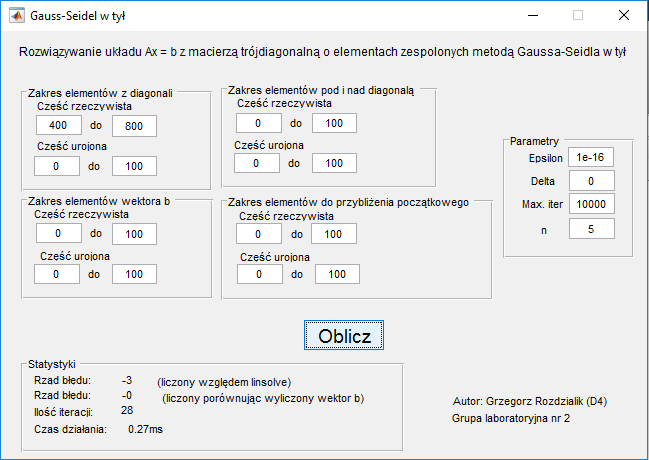
\includegraphics[scale=0.8]{gui-image}
	
	Interfejs graficzny jest graficzną wersją skryptu testującego \textit{testScript.m} i pokazuje następujące wyniki:
	\begin{itemize}
		\item rząd błędu rozwiązania obliczonego za pomocą $linsolve$ dostępnego w Matlabie oraz czas działania tych obliczeń (w milisekundach)
		\item rząd błędu liczony względem wektora $b$ ($\|Ax - b\|$)
		\item ilość iteracji
		\item czas działania metody Gaussa-Seidla w tył (w milisekundach)
	\end{itemize}

	\pagebreak

	\section{Bibliografia}
	\begin{itemize}
		\item \href{https://pl.wikipedia.org/wiki/Metoda_Gaussa-Seidla}{Metoda Gaussa-Seidla - Wikipedia, wolna encyklopedia}
		\item P. Tatjewski \textit{Metody numeryczne}, Warszawa: Oficyna Wydawnicza PW, 2013
	\end{itemize}
\end{document}